%   packages:
\documentclass{article}
\usepackage[utf8]{inputenc}
\usepackage[T1]{fontenc}
\usepackage{microtype}
\usepackage{graphicx}
\usepackage{fancyhdr}
\usepackage{float}
\usepackage{lipsum}
\usepackage{newspaper}
\usepackage{newspaper-mod}
\usepackage{multicol}
\usepackage{picinpar}

% uasage of picinpar:
% \begin{window}[1,l,\includegraphics{},caption]xxxxx\end{window}

% These can be issued just before any
% byline or headline in the paper, to
% individually style each article
% \renewcommand{\headlinestyle}{\itshape\Large\lsstyle}
% \renewcommand{\bylinestyle}{\bfseries\Large\raggedright}


% TODO: Change the font to Times New Roman

\setlength{\parindent}{2pt}
%To get rid of indents 


%Metadata you shouldn't change
\SetPaperName{
          %  
\includegraphics[scale=0.3]{fps}
        % \scalerel*{
\includegraphics{fps}}{f}
            FPS Eagles:   
         \hfill  \includegraphics[scale=0.1]{mascot} 
      }
\SetHeaderName{FPS Eagles}
\SetPaperLocation{
%    \centering
   %\begin{figure}
    %   \centering
  %  \vspace{5mm}
  %  
\includegraphics[scale=0.12]{lfps} 
   %  
\includegraphics[scale=0.09]{W}
   %\end{figure}
    
   
}
\SetPaperSlogan{
            %     
\includegraphics[scale=0.3]{fps}
        %        FIRST ISSUE!
                
                ``\textit{FPSonians are the best; second to none!}''
              %  
\includegraphics[scale=0.1]{cfps}
                }
\SetPaperPrice{By Awab Qureshi and Sukaina Kazmi; batch 2020}
%\cfoot{\textit{First issue ever! FPSonians are the best; second to none!}}




% Metadata you should change
\date{January 2020}
\currentvolume{1}
\currentissue{1} 




\begin{document}
\maketitle
\large 

%                               1ST PAGE

\headline{MAIN}\textbf{by} % 200~250 words


%do \closearticle for that double line bar

\begin{multicols}{2}
%to make columns

\includegraphics[scale=0.2]{w}

Pic of main goes here
% \includegraphics[scale=0.5]{picture of main}

\includegraphics[scale=0.1]{w}


\headline{Side 1}\textbf{by} % 140~150 words





\end{multicols}
\pagebreak 

%to make sure stuff stays on this page

%                               2ND PAGE 

\headline{Editorial}\textbf{by} % 350 words



\closearticle

\begin{multicols}{2}
\headline{Sports} % 130 words





\begin{center}
    % \includegraphics[scale=0.4]{}    
    Pic for sports here
\end{center}


%\headline{This Week in History}




\end{multicols}

\closearticle

\pagebreak


%                               3RD PAGE

\headline{What's Up With Tech?}
\begin{multicols}{2}
    \headline{tech 1} % 100 words

%\closearticle


\headline{tech 2} % 100 words

%\vfill
%\closearticle

\end{multicols}
\closearticle

\begin{center}
\headline{Jokes, and Memes}
%
\includegraphics[height=5.5cm]{m1.jpeg}
%
\includegraphics[height=5.5cm]{m2.jpeg}
Memes here
%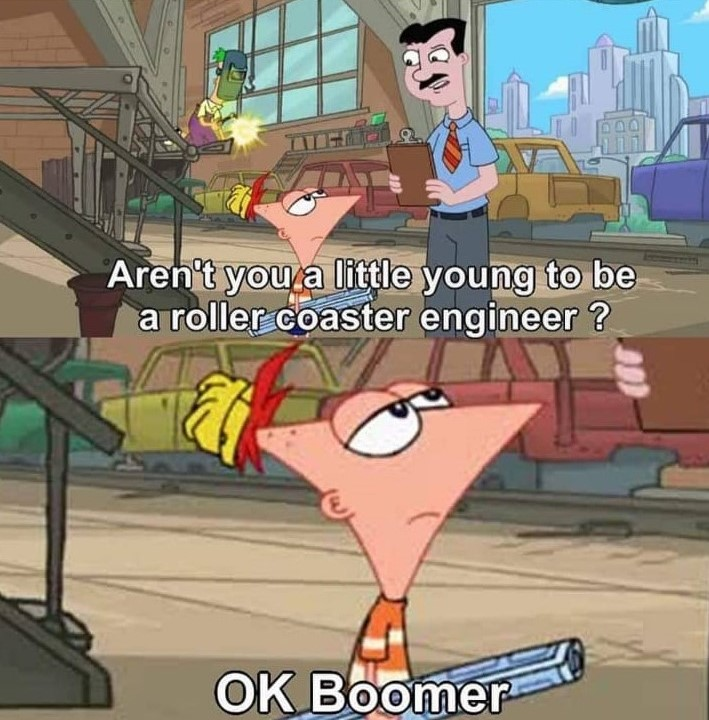
\includegraphics[height=6cm]{m3.jpeg}
%
\includegraphics[height=6cm]{m4.jpeg}
\end{center}

\pagebreak


%                               4TH PAGE

\begin{multicols}{2}

\headline{misc 1} % 190 words



\includegraphics[scale=0.1]{w}
\vfill

% 
\includegraphics[scale=0.39]{grammy}
Image for misc 1 here


\headline{Misc 2?} % 190 words

%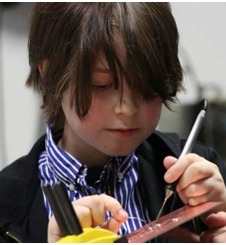
\includegraphics[scale=1]{prodigy}
Image for misc 2 here

\pagebreak


\end{multicols}


\end{document}